\chapter*{6. Estimación y resultados}

\section*{6.1. Estimación de demanda con variables instrumentales}

La ecuación de demanda agregada busca capturar las principales fuerzas económicas que determinan el precio y las cantidades comercialziadas en el mercado internacional del café:

\begin{equation}
    Q_{t} = \alpha^{d}_{0} + \alpha^{d}_{1}P_{t} + \alpha^{d}_{2}X_{t} + \alpha^{d}_{3}Z{t} + \alpha^{d}_{4} ICA_{t} + u^{d}_{t}
\end{equation}

La variable dependiente $Q_{t}$ refleja la cantidad total demandada en el mercado, mientras que $P_{t}$ representa el índice global de precios. Por otro lado, la inclusión de $X_{t}$, el Producto Interno Bruto (PIB) de los países importadores, permite medir la sensibilidad del consumo frente a cambios en el poder adquisitivo de este grupo.

Se incluye también el precio del té ($Z_{t}$) en la estimación, reconociendo que, aunque no son perfectos sustitutos, existen márgenes de sustitución que pueden influir en la demanda de café, especialmente en períodos de altos precios. 

Para controlar por el período en que el mercado estuvo cartelizado, se incorpora una variable dicotómica que toma el valor 1 desde enero de 1990 ($ICA_{t}$). Por su parte, el término error ($u^{d}_{t}$) recoge factores no observables, como cambios en las preferencias de consumo o efectos estacionales no modelados explícitamente.

Esta especificación sigue el enfoque de los trabajos seminales de [KARL PERLOFF] e [IGAMI]. Al mantener esta estructura, los resultados obtenidos permiten comparaciones directas con los hallazgos de esos estudios, facilitando la evaluación de consistencia en las elasticidades-precio estimadas y su evolución temporal. Así también, para resolver el problema de agregación temporal entre variables mensuales y anuales, se adopta la forma funcional de la demanda inversa:

\begin{equation}
    P_{t} = \frac{1}{\alpha^{d}_{1}} \left[ Q_{t} - ( \alpha^{d}_{0} + \alpha^{d}_{2}X{t} + \alpha^{d}_{3}Z{t} + \alpha^{d}_{4} ICA_{t} + u^{d}_{t} ) \right]
\end{equation}

Naturalmente, la identificación causal de la relación entre la cantidad demandada y el índice global de precios requiere abordar el problema de endogeneidad mediante la aproximación de variables instrumentales. En esta investigación, se selecciona la variable \textit{HDD} por su relación con las variaciones exógenas en la oferta global del café, lo que permitiría que satisfaga los requisitos de relevancia y exogeneidad. Más adelante, esta variable serán fundamental para la estimación de los costos marginales implícitos y la construcción de escenarios contrafactuales, dado su vínculo con los determinantes de la oferta.

Explicada en detalle en \textit{supra}, esta variable cuantifica, para cada mes, la exposición a condiciones de temperatura adversas para el cultivo del café. Para esta estimación, se agrega la variable a nivel global mediante ponderaciones basadas en la participación de mercado histórica de cada exportador.

Se espera que, por la relación de esta variable con la oferta del grano del café, satisfaga con éxito las condiciones de exogeneidad y relevancia que exige el uso de variables instrumentales. Como se verá, las pruebas de sobreidentificación (Hansen J) y los diagnósticos de debilidad instrumental (estadístico F de Cragg-Donald) confirman su adecuación empírica.

La \ref{tab:7_1} presenta los resultados de la estimación de demanda a nivel mensual, tomando información desde 1965 hasta 2019. En todas las especificaciones se controla por el período de cartelización del mercado. Los modelos 1, 2 y 3 solo consideran variables de control, mientras que los modelos 4, 5 y 6 incluyen las variables instrumentales discutidas en esta sección.

Se obtienen resultados similares al trabajo de Igami (ver anexo XXX) aunque con algunos matices, posiblemente explicados por la diferencia en el horizonte temporal \footnote{Las estimaciones de demanda agregada de este trabajo abarca un extenso período desde 1965 hasta 2019, mientras que Igami toma un horizonte más acotado, desde 1990 hasta 2006.} o por el control para el período de cartelización. En particular, este trabajo presenta un impacto similar de la cantidad exportada, mientras que los efectos del ingreso y del bien sustituto son mayores.

En concreto, por cada aumento de un millón de bolsas de 60 kg de café, el precio cae en 215 centavos de dólar, relativamente cercano a los 293 obtenidos por Igami. Asimismo, la elasticidad-precio de la demanda estimada para este trabajo está en un rango aceptable, indicando una demanda inelástica, pese a las fluctuaciones de precio\footnote{Igami obtiene una elasticidad-precio de la demanda de 0,15. Por su parte, otros trabajos han obtenido resultados de 0,2, al igual que en este caso. Ver, por ejemplo, \cite{bates1997open}.}. Esta demanda inelástica, en conjunto con la existencia de choques climáticos importantes, es consistente con la explicación estándar para la variación de los precios de los bienes agrícolas (\cite{deaton1992behaviour}, \cite{prebisch1959}, \cite{singer1950}).

\begin{table}[!htbp] \centering 
\caption{Estimaciones de la Demanda Mundial de Café} 
\label{tab:7_1}
 \resizebox{0.85\textwidth}{!}{
\begin{tabular}{@{\extracolsep{5pt}}lcccccc} 
\hline 
\hline 
 & \multicolumn{3}{c}{\textit{MCO}} & \multicolumn{3}{c}{\textit{VI}} \\ 
\cline{2-7} 
Var. dep.: $P_{t}$ (Precio) & (1) & (2) & (3) & (4) & (5) & (6)\\ 
\hline 
 $Q_{t}$ (Exportaciones de café) & $-$16.396$^{***}$ & $-$102.711$^{***}$ & $-$130.271$^{***}$ & $-$176.303$^{***}$ & $-$362.252$^{***}$ & $-$294.519$^{***}$ \\ 
  & (3.529) & (13.641) & (9.978) & (29.619) & (32.086) & (16.126) \\ 
  & & & & & & \\ 
 $ICA$ ($0/1$) & $-$190.547$^{***}$ & $-$300.680$^{***}$ & $-$202.651$^{***}$ & 233.023$^{***}$ & $-$405.657$^{***}$ & $-$244.207$^{***}$ \\ 
  & (9.711) & (19.152) & (13.622) & (74.874) & (30.169) & (18.625) \\ 
  & & & & & & \\ 
 $X_{t}$ (PIB de importadores) &  & 322.739$^{***}$ & 472.105$^{***}$ &  & 1,077.710$^{***}$ & 965.645$^{***}$ \\ 
  &  & (42.679) & (36.825) &  & (93.878) & (48.985) \\ 
  & & & & & & \\ 
 $Z_{t}$ (Precio del té) &  &  & 0.783$^{***}$ &  &  & 0.961$^{***}$ \\ 
  &  &  & (0.081) &  &  & (0.054) \\ 
  & & & & & & \\ 
 Constante & 447.166$^{***}$ & 653.794$^{***}$ & 292.019$^{***}$ & 1,231.079$^{***}$ & 1,419.667$^{***}$ & 675.726$^{***}$ \\ 
  & (24.053) & (45.787) & (30.288) & (149.459) & (99.642) & (49.066) \\ 
  & & & & & & \\ 
\hline 
Observations & 658 & 658 & 658 & 658 & 658 & 658 \\ 
R$^{2}$ & 0.509 & 0.591 & 0.755 & - & 0.012 & 0.532 \\ 
Adjusted R$^{2}$ & 0.507 & 0.589 & 0.754 & - & 0.008 & 0.529 \\ 
Residual Std. Error & 115.702 (df = 655) & 105.643 (df = 654) & 81.777 (df = 653) & 200.914 (df = 655) & 164.214 (df = 654) & 113.070 (df = 653) \\ 
F Statistic & 339.273$^{***}$ (df = 2; 655) & 315.201$^{***}$ (df = 3; 654) & 504.128$^{***}$ (df = 4; 653) &  &  &  \\ 
\hline 
\hline 
\textit{Note:}  & \multicolumn{6}{r}{Errores estándar robustos clusterizados por año entre paréntesis.} \\ 
 & \multicolumn{6}{r}{$^{*}$p$<$0.1; $^{**}$p$<$0.05; $^{***}$p$<$0.01} \\ 
\end{tabular}}
\end{table} 

[Sobre los instrumentos]

Una vez estimada la ecuación de demanda, recuperar el coeficiente $\hat{\alpha}^{d}_{1}$ permite estimar los costos marginales de cada país ($c{i,t}$), siguiendo las ecuaciones (5) y (6).

\section*{6.2. Estimación de costos marginales}

La estimación del impacto del cambio climático sobre los costos marginales del modelo se lleva a cabo en dos etapas. Primero, se computan los costos marginales implícitos de la estimación de demanda siguiendo las ecuaciones (5) y (6). Luego, se estima el efecto de los factores de costo y choques climáticos siguiendo la siguiente especificación:

\begin{equation}
    c_{i,t} = \alpha^{o}_{0} + 
\alpha^{o}_{1}F_{t} +
\alpha^{o}_{2}HDD_{t} +
\alpha^{o}_{3}FDD_{t} +
\alpha^{o}_{4}ICA_{t} +
\phi_{i}+\phi_{t}+u^{o}_{i,t}
\end{equation} 

donde $F_{t}$ es el índice de precios de fertilizantes calculado por el Banco Mundial, $HDD_{t}$ es la acumulación de calor, explicada \textit{supra}, $FDD_{t}$ es la acumulación de frío extremo, también explicada, $ICA_{t}$ es una variable dicotómica para el período de cartelización, $\phi_{i}$ es un efecto fijo por país, $\phi_{t}$ es un efecto fijo por año y $u^{o}_{i,t}$ es el término error.

La [TABLA] resume los resultados para la especificación utilizada. Se observa que el impacto de las variables asociadas a la acumulación de temperaturas extremas es bastante relevante. En particular, la variable $FDD$ indica un efecto de 74 centavos de dólar sobre los costos marginales, mientras que $HDD$ tendría un efecto menor, de 12 centavos. En ambos casos, la significancia es máxima. Por otro lado, el ajuste $R^{2}$ indica que el modelo explica gran parte de la variación del error. 

Por otro lado, si separamos la muestra a fin de observar específicamente el efecto de estas variables climáticas sobre países lídere y seguidores, se observa que el impacto es notablemente mayor para el segundo grupo. Así, como se desarrollará con detalle en el análisis de los resultados contrafactuales, el impacto del cambio climático afectaría más a aquellos países que actúan como seguidores del mercado. En el caso de la acumulación de frío, el efecto sería un 24\% más importante para el grupo de seguidores; mientras que la diferencia en la acumulación de calor asciende hasta un 38\% aproximadamente.

\input{tables/t6_01.tex}

\section*{6.3. Ajuste del modelo y escenarios contrafactuales}
A partir de los resultados obtenido hasta ahora, es posible identificar la sensibilidad de la demanda ante los choques de precios y computar los costos marginales del sistema. Junto con la interacción estratégica de los agentes, es directo estimar el escenario factual, y revisar así el ajuste del modelo a los datos observados.

Las [FIGURAS] muestran el ajuste de la estimación para el precio y las cantidades observadas. Es directo ver que la estimación estructural permite identificar buena parte de la evolución de ambas series. En promedio, la diferencia entre los valores observados y la predicción del modelo es de un 4\% para el precio y de un 0,9\% para las exportaciones.

\begin{figure}[H]
    \centering
    \caption{Precio observado y estimado}
        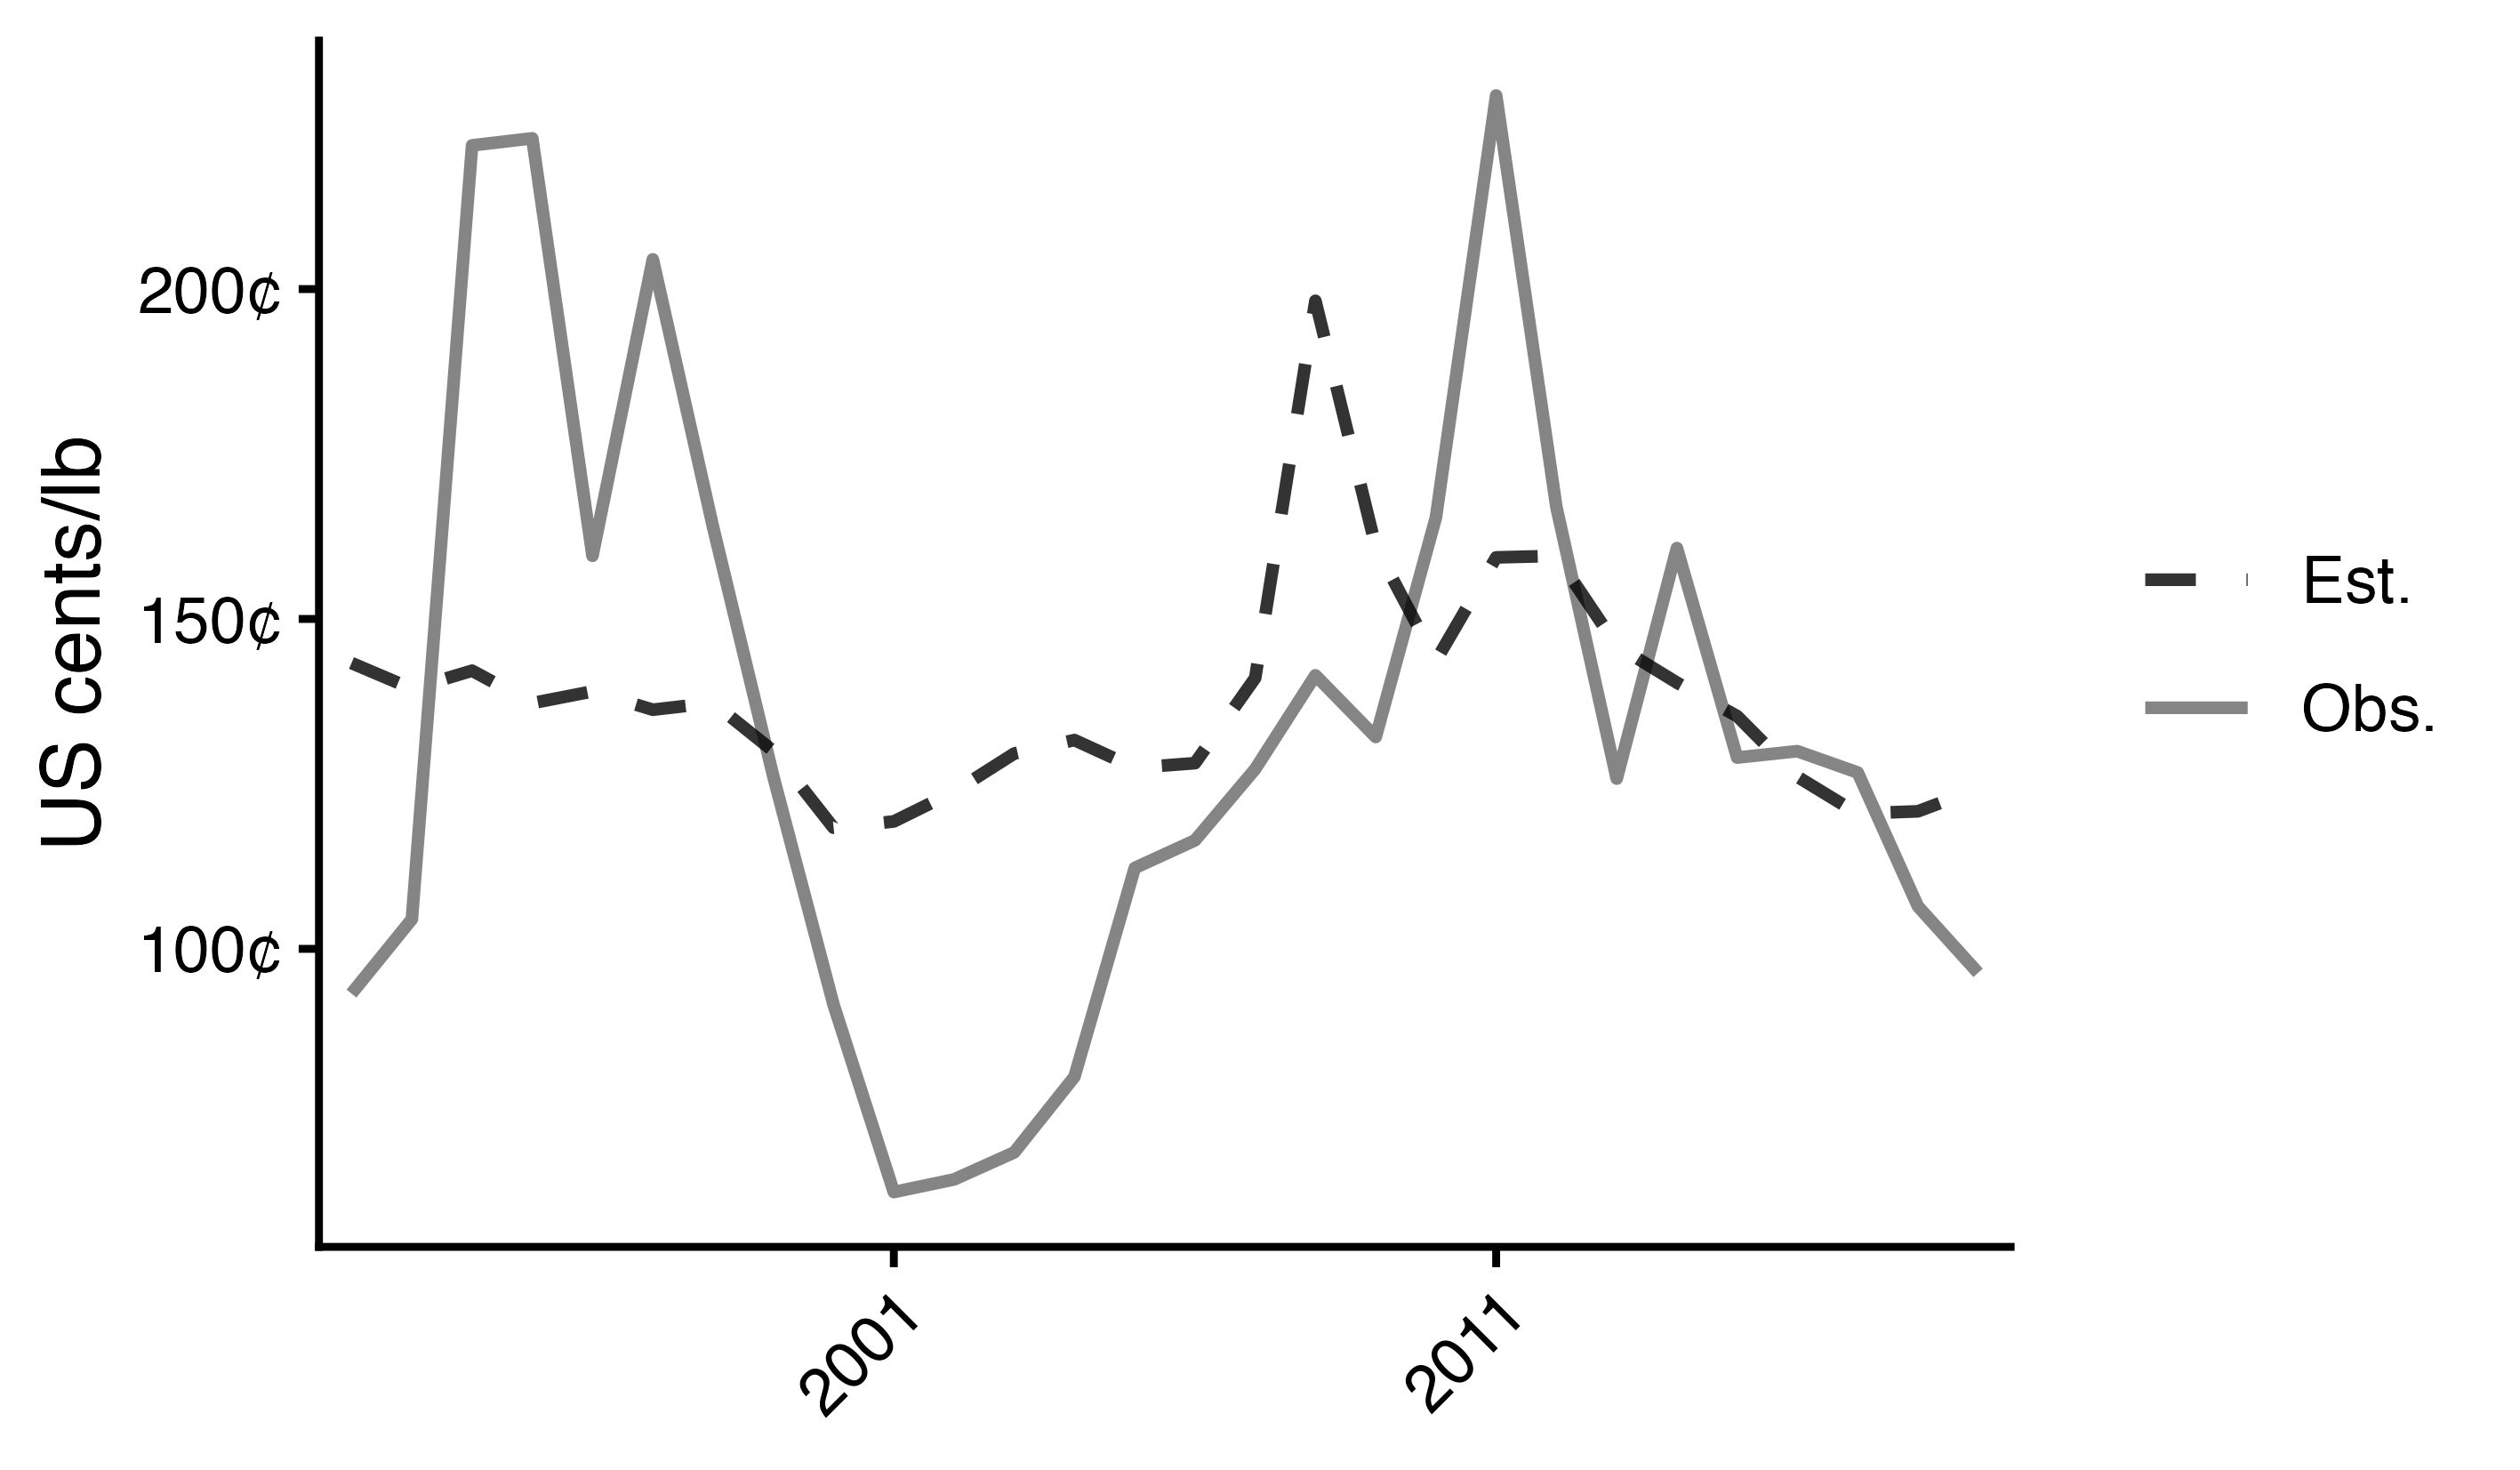
\includegraphics[scale = 0.9]{figures/plot_0601.png}
        \label{fig:plot06_01}
\end{figure}

\begin{figure}[H]
    \centering
    \caption{Exportaciones observadas y estimadas}
        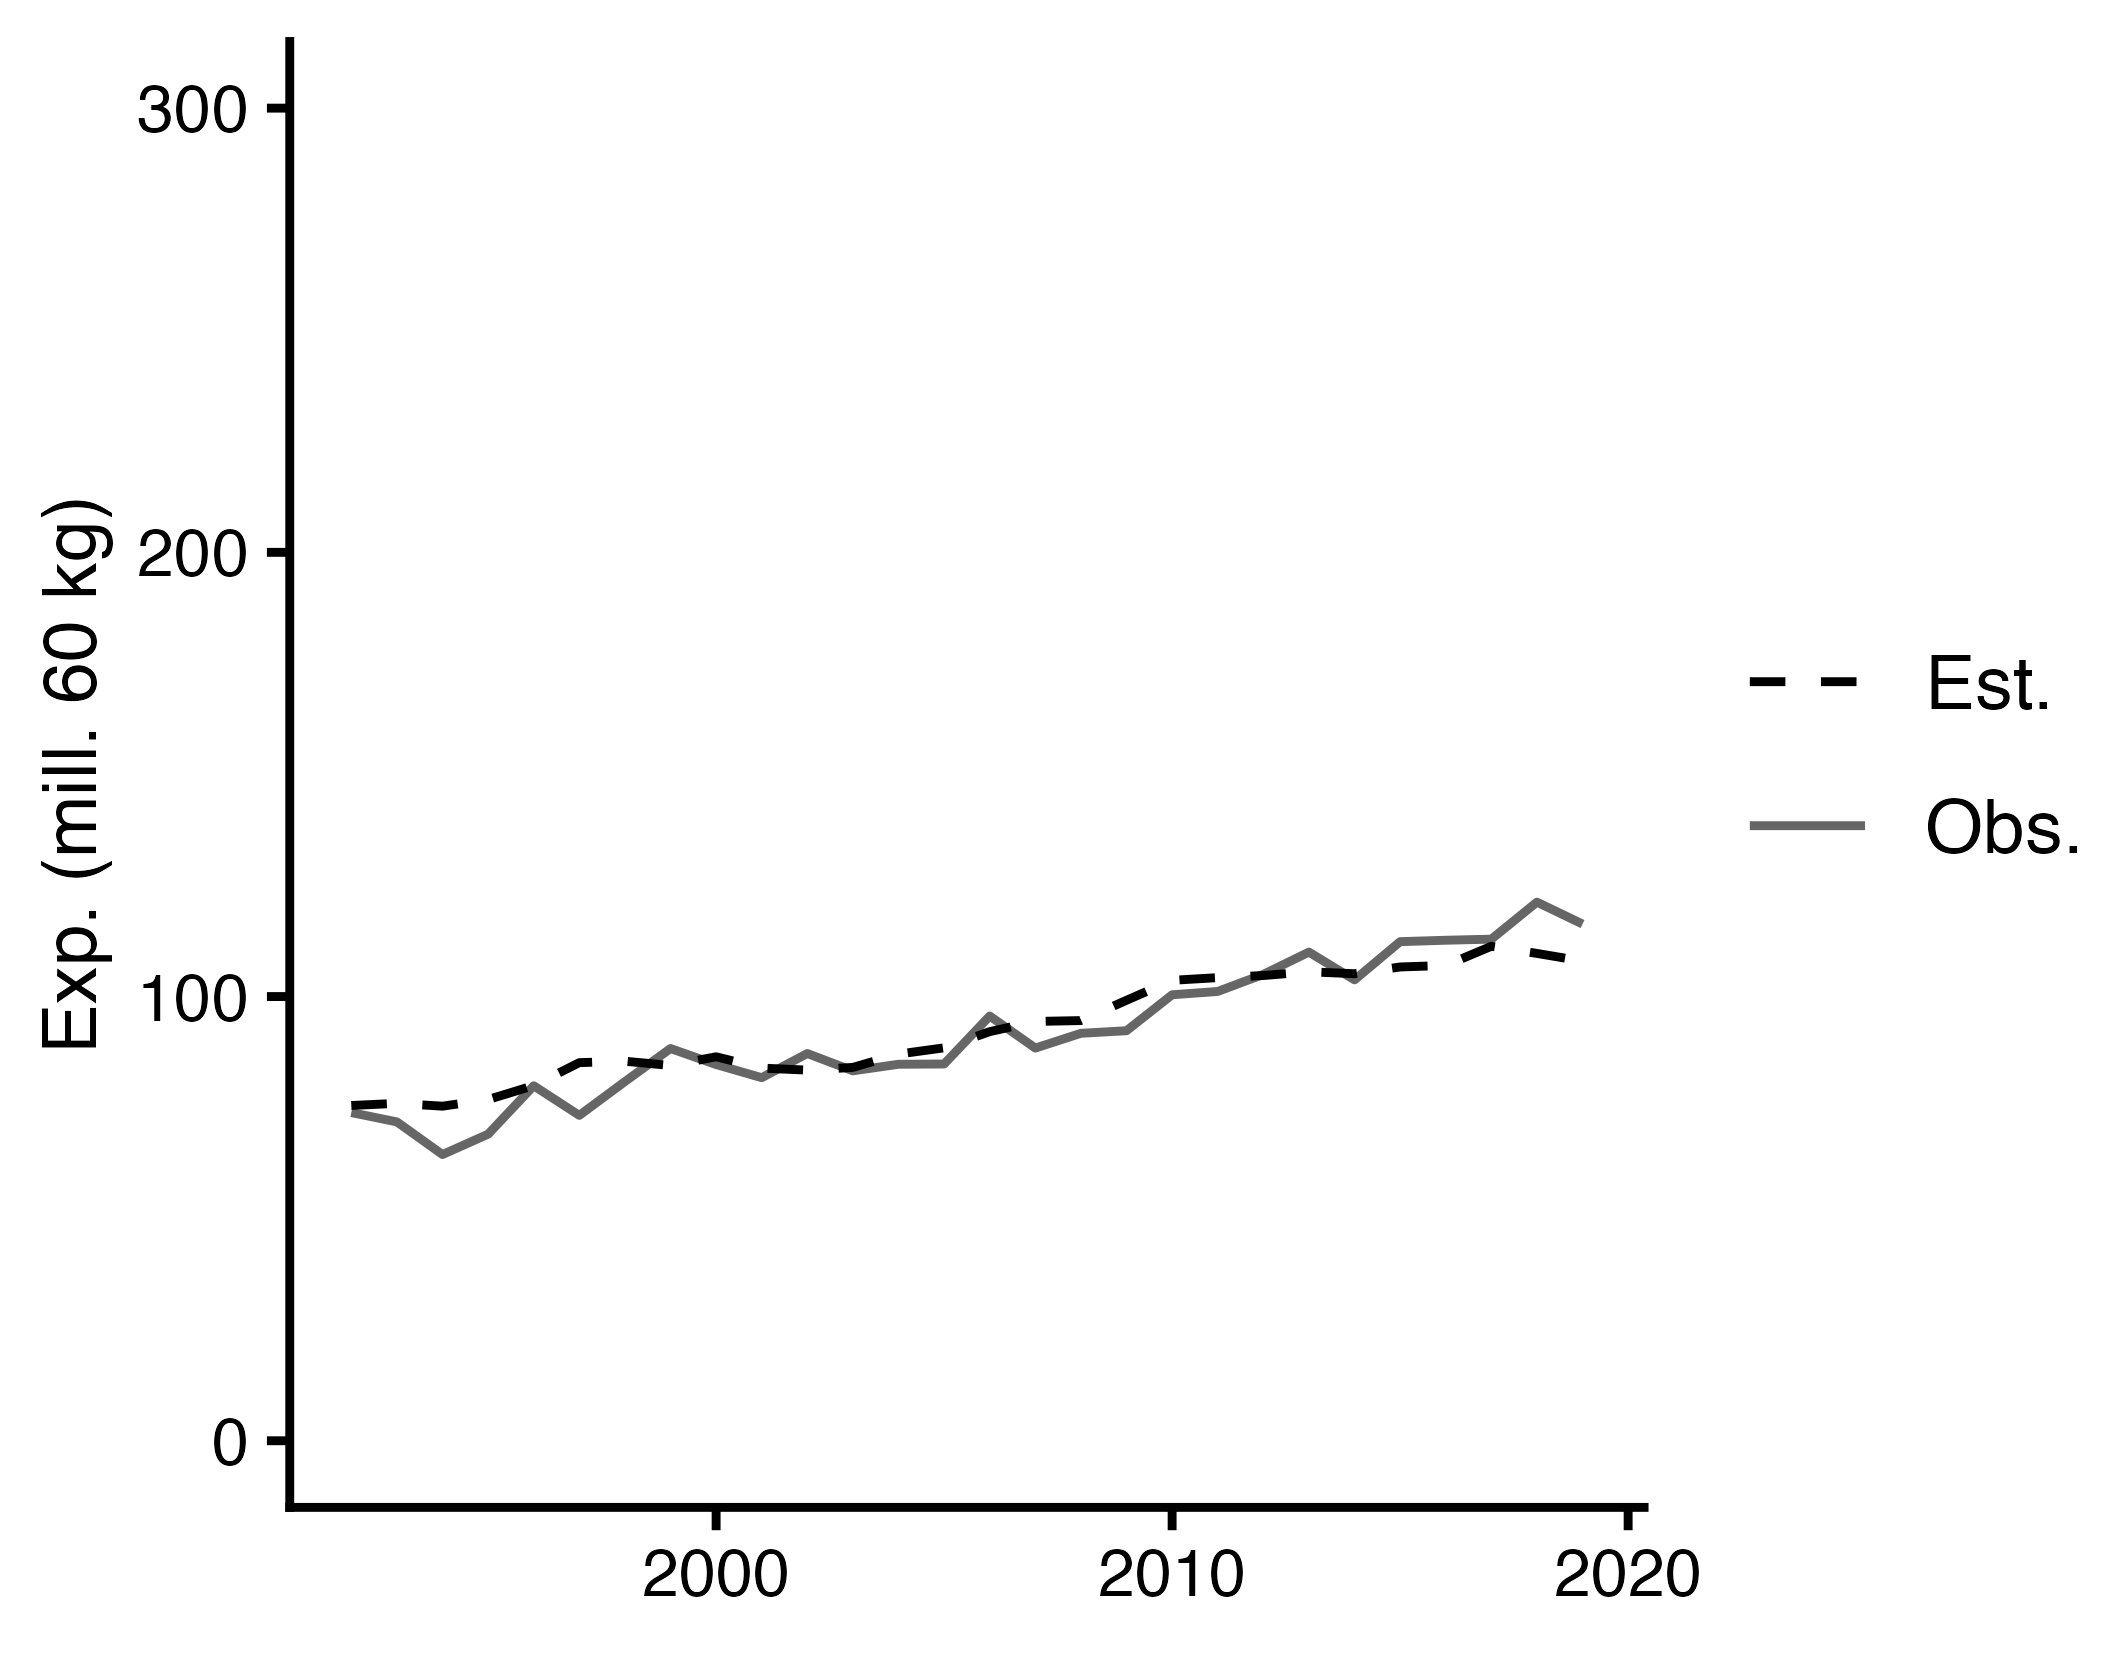
\includegraphics[scale = 0.9]{figures/plot_0602.png}
        \label{fig:plot06_02}
\end{figure}

Ahora bien, uno de los principales objetivos de esta investigación es la estimación de escenarios contrafactuales en el mercado internacional del café. En particular, interesa analizar el cambio en la trayectoria de precios y cantidades comercializadas una vez que se reduce el estrés térmico, modificando las variables climáticas relevantes en tal sentido. Luego, a partir de estos resultados, es posible calcular el efecto en el bienestar social, así como diferencias entre grupos de exportadores. Esta última distinción permitiría explorar si acaso el estrés térmico amplifica las diferencias estructurales entre países líderes y seguidores.

Las [TABLAS] presentan los resultados para diferentes escenarios contrafactuales, bajo reducciones en la exposición a temperaturas extremas. El primer caso (Contrafactual 1) se obtiene de reducir en un 25\% la exposición mensual de cada país, tanto a temperaturas altas (sobre 30°C) como a temperaturas bajas prolongadas (bajo 10°C). El segundo caso (Contrafactual 2) se obtiene luego de reducir en un 50\% la exposición. El último escenario (Contrafactual 3) es aquel que no presenta exposición a temperaturas extremas.

La [TABLA] muestra que, en general, las reducciones en la exposición tiene consecuencias importantes sobre el precio y las cantidades exportadas, aunque la magnitud de tal efecto pareciera no ser tan alta. Así, las reducciones van de un 1,2\% a un 4,9\% en el caso del precio y de un 0,2\% a un 0,8\% para las exportaciones, de manera que la exposición afectaría más al índice global del \textit{soft commodity} que a las decisiones de exportación de los agentes. Esto es muy importante, pues el mecanismo mediante el cual el estrés térmico afecta al mercado internacional del café no es evidente; los resultados sugieren que la volatilidad del precio y su susceptibilidad a choques climáticos es clave.

Por otro lado, la [TABLA] presenta los resultados en términos de bienestar, para los diferentes grupos de interés en el sistema. Como se puede observar, quienes pierden mayor excedente, en promedio, son los líderes del mercado; el impacto va de un 0,6\% en un escenario con 25\% de reducción del estrés térmico, a un 2,3\% en un escenario sin estrés térmico. Enseguida, el grupo de importadores presenta un impacto que va del 0,4\% a un 1,7\%; luego, los seguidores registran un impacto del 0,2\% a un 1\% en su excedente.

Con todo, se debe tener presenta que lo anterior solo refleja el impacto de reducir la exposición sobre el excedente de cada grupo, a nivel agregado, mas no permite identificar si existen diferentes mecanismos a través de los cuales el estrés térmico materializa su efecto. 

\begin{table}[H]
\centering
\caption{Estimación de un escenario sin estrés térmico. Resultados de precios y cantidades.}
\label{tab:t6_results}
\begin{tabular}{lcc}
\hline
\textbf{Escenario} &
  \textbf{\begin{tabular}[c]{@{}c@{}}Precio\\ (¢)\end{tabular}} &
  \textbf{\begin{tabular}[c]{@{}c@{}}Exportaciones\\ (mill. 60 kg.)\end{tabular}} \\ \hline
Factual &
  147 &
  4.871\\
Contrafactual &
  141 ($\downarrow$ 4,6\%) &
  4.881 ($\uparrow$ 0,2\%) \\ \hline
\end{tabular}%
\end{table}

\begin{table}[H]
\centering
\caption{Estimación de un escenario sin estrés térmico. Resultados de excedente social.}
\label{tab:t6_surplus}
\resizebox{\textwidth}{!}{
\begin{tabular}{lcccc}
\hline
\textbf{Escenario} &
  \textbf{\begin{tabular}[c]{@{}c@{}}Excedente\\ líderes\end{tabular}} &
  \textbf{\begin{tabular}[c]{@{}c@{}}Excedente\\ seguidores\end{tabular}} &
  \textbf{\begin{tabular}[c]{@{}c@{}}Excedente\\ importadores\end{tabular}} &
  \textbf{\begin{tabular}[c]{@{}c@{}}Excedente\\ total\end{tabular}} \\ \hline
Factual &
  56.481 &
  85.206 &
  10.031.905 &
  10.173.592 \\
Contrafactual 1 &
  55.958 ($\downarrow$ 0,9\%) &
  87.279 ($\uparrow$ 2,4\%) &
  10.076.983 ($\uparrow$ 0,5\%) &
  10.220.220 ($\uparrow$ 0,5\%)  \\ \hline
\end{tabular}
}
\end{table}

Con el objetivo de identificar con mayor detalle si existen diferencias en el impacto del estrés térmico sobre los líderes y seguidores del sistema, se plantea la siguiente regresión sobre variables dicotómicas:

\begin{equation}
    \centering
    x_{i,t} = \beta_{1} \text{Contrafactual} + \beta_{2} \text{Líderes}  + \beta_{3} \text{Contrafactual} \times \text{Líderes} + e_{i,t} 
\end{equation}

donde $\hat{x}_{i,t}$ es la variable de interés, que puede referirse a los costos ($\hat{c}_{i,t}$), exportaciones ($q_{i,t}$) o beneficios ($\pi_{i,t}$). Por otro lado, $\text{Contrafactual}$ y $\text{Líderes}$ son variables dicotómicas que toman el valor 1 si corresponde al escenario contrafactual o a líderes, respectivamente. El coeficiente de interés para este análisis es aquel asociado a la intersección de las variables explicativas anteriores, pues refleja si existe un efecto diferencial entre escenarios por el solo hecho de pertenecer a un determinado grupo exportador.

Los resultados muestran que este efecto diferencial existe y es significativo estadísticamente, de manera que, para todas las variables analizadas, el estrés térmico sí afecta las diferencias estructurales ya presentes en el mercado. 

Primero, en cuanto a los costos marginales del sistema, se puede observar que el escenario contrafactual efectivamente reduce los costos marginales de ambos grupos. El efecto es equivalente a [XXXX], sobre una variable que toma un valor promedio de [XXXX]. Luego, los costos serían, en promedio, mayores para los líderes del mercado [Revisar esto]. Por último, se observa un efecto diferencial negativo, es decir, el escenario contrafactual implica una mayor reducción del costo marginal para los grandes exportadores.

Segundo, los resultados sobre las cantidades exportadas reafirman la idea de que el escenario contrafactual no implica mayores cambios. Por otro lado, en promedio, los países líderes exportan más que los seguidores del sistema. El efecto diferencial, aunque pequeño, existe y es significativo, y va en la dirección del contrafactual.

\begin{table}[H]
   \caption{Escenario contrafactual. Efecto diferencial de líderes.}
   \bigskip
   \centering
   \begin{tabular}{lccc}
      \hline 
      \hline 
      \toprule
                            & $c_{i, t}$ & $q_{i, t}$       & $\pi_{i, t}$ \\   
                            & (1) & (2)           & (3)\\  
      \hline
      \midrule 
      Efecto             & -117.27$^{***}$ & 0.01$^{***}$ & 0.54$^{***}$\\   
      Contrafactual ($\beta_{1}$) & (3.73) & (0.0005)       & (0.09)\\   
      Efecto  & 217.41$^{***}$ & 11.88$^{**}$  & 229.66$^{***}$\\   
      Líderes ($\beta_{2}$) & (38.43) & (0.7436) & (52.57)\\   
      Efecto      & -7.04$^{**}$ & 0.16$^{***}$  & 6.02$^{***}$\\   
      Diferencial ($\beta_{3}$) & (2.63) & (0.0070)        & (1.25)\\
       \\
      \hline
      Observaciones          & 3.408 & 3.408 & 3.408 \\  
      R$^2$                 & 0,9768 & 0.7747 & 0.4900\\  
       \\
   \end{tabular}
\end{table}

[RESULTADOS ENTRE EXPORTADORES E IMPORTADORES]
[RESULTADOS DENTRO DE CADA GRUPO]
[RESULTADOS POR LATITUD Y LONGITUD. MAPA MUNDIAL CON RESULTADOS]